\RequirePackage{amsmath}
\documentclass[twocolumn, times]{aastex63}
\usepackage[spanish,es-minimal,english]{babel}
\usepackage[utf8]{inputenc}
\usepackage{natbib}
%\usepackage{microtype}
\usepackage{hyperref}
\usepackage{savesym}
\savesymbol{tablenum}
\usepackage{siunitx}
\restoresymbol{SIX}{tablenum}
\usepackage[varg]{newtxmath}
\usepackage{newtxtext}
\usepackage{booktabs}
\usepackage{array}   % for \newcolumntype macro
\newcolumntype{L}{>{$}l<{$}} % math-mode version of lrc column types
\newcolumntype{R}{>{$}r<{$}} 
\newcolumntype{C}{>{$}c<{$}} 

\bibliographystyle{aasjournal}

\graphicspath{ {../paper/} }

\newcommand\ION[2]{#1\,\scalebox{0.9}[0.8]{\uppercase{#2}}}
\newcounter{ionstage}
\renewcommand{\ion}[2]{\setcounter{ionstage}{#2}% 
  \ensuremath{\mathrm{#1\,\scriptstyle\Roman{ionstage}}}}
\newcommand\hii{\ion{H}{2}}
\newcommand\Raman{\ensuremath{_{\text{Raman}}}}
\def\th#1#2{\(\theta^{#1}\)\,Ori~#2}
\newcommand\wn{\ensuremath{\tilde{\nu}}}

% Chemical formulae
\newcommand*\chem[1]{\ensuremath{\mathrm{#1}}}
% Atomic term symbols
\newcommand\Config[1]{\ensuremath{\mathrm{#1}}}
\newcommand\Term[3]{\ensuremath{\mathrm{#1\ ^{#2}#3}}}
\newcommand\Level[4]{\ensuremath{\mathrm{#1\ ^{#2}#3_{#4}}}}

\newcommand\ha{\ensuremath{\text{H}\alpha}}
\newcommand\lya{\ensuremath{\text{Ly}\alpha}}
\newcommand\lyb{\ensuremath{\text{Ly}\beta}}
\newcommand\FUV{\ensuremath{_{\text{FUV}}}}

\begin{document}
\title{On the geometry of the Orion Bar}
\shorttitle{Orion Bar geometry}
\author{William J. Henney}
\affiliation{%
  \foreignlanguage{spanish}{Instituto de Radioastronomía y
    Astrofísica, Universidad Nacional Autónoma de México, Apartado
    Postal 3-72, 58090 Morelia, Michaoacán, Mexico}}
\email{w.henney@irya.unam.mx}

\begin{abstract}
  I critically examen different geometrical models that have been proposed for the
  geometry of the Orion Bar photodissociation region.
  From a re-analysis of the of the \SI{21}{cm} \ion{H}{1} observations,
  I show that the ionization front at the Bar must be convex,
  which rules out important classes of models.
  Furthermore, I show that small scale irregularities in the
  ionization front and dissociation front are important for
  analysing the apparent stratification and widths of different emission regions.
\end{abstract}

\keywords{Atomic physics; Radiative transfer; Photodissociation regions}
%\facilities{VLT:Yepun (MUSE); VLA}
%\object{M42}

\newcommand\vdw{vdW13}
\newcommand\vlsr{\ensuremath{v_{\mathrm{lsr}}}}
\section{Reanalysis of \SI{21}{cm} \ion{H}{1} observations of the Orion Bar}
\label{sec:reanalysis-21-cm}

Karl G.\ Jansky Very Large Array observations of the \ion{H}{1}
\SI{21}{cm} line from the Orion Nebula and its surroundings at a
spatial resolution of \(\approx 6''\) and a velocity resolution of
\SI{0.77}{km.s^{-1}} were presented in \citet[hereafter
vdW13]{van-der-Werf:2013a}.  The line is seen both in emission and
absorption of the strong free-free continuum emitted by the ionized
nebula.  The majority of the absorption arises in the foreground Veil
at Local Standard of Rest velocities of
\(\vlsr = \text{\SIrange{-2}{+7}{km.s^{-1}}}\). Emission is seen
primarily at more redshifted velocities of
\SIrange{+10}{+15}{km.s^{-1}}, similar to the velocities of the
molecular gas seen in CO, although at large distances from the center
of the nebula the Veil is also seen in emission.  The analysis of the
absorption components by \vdw{} was carried out under the assumptions
that (i)~all of the continuum emission arises from \emph{behind} the
absorbing \chem{H^0} column (from the point of view of the Earth), and
(ii)~line emission is negligible at velocities where absorption is
detected.  These are both very good assumptions in the case of
absorption by the foreground Veil, but they break down for the case of
the Orion Bar, where both emission and absorption are seen at similar
velocities and in spatially adjacent regions.  Given the wealth of
information on the physical conditions and geometry that these data
provide, it is worth reanalyzing them under less restrictive
assumptions.

\newcommand{\Ttb}{\ensuremath{\tilde{T}_{\mathrm{b}}}}
\newcommand{\Tb}{\ensuremath{T_{\mathrm{b}}}}
\newcommand{\Tc}{\ensuremath{{T_{\mathrm{c}}}}}
\newcommand{\Te}{\ensuremath{T_{\mathrm{e}}}}
\newcommand{\Ts}{\ensuremath{T_{\mathrm{s}}}}

\begin{figure}
  \centering
  \caption{Three-layer sandwich structure for \ion{H}{1} \SI{21}{cm} radiative transfer.}
  \label{fig:hii-hi-hii-sandwich}
\end{figure}

In the Rayleigh--Jeans limit, the frequency-dependent surface
brightness \(I_\nu\) is characterized by the brightness temperature in
each velocity channel: \(T_{\mathrm{b}}(v) = c^2 I_\nu / 2 k \nu^2\),
where \(v/c = (\nu/\nu_0) - 1\) and \(\nu_0 = \SI{1.420405}{GHz}\).  The
radiative transfer equation can be solved for an idealized three-layer
sandwich structure (see Fig.~\ref{fig:hii-hi-hii-sandwich}),
consisting of (1)~a background \chem{H^+} region with electron
temperature \Te{} and free-free continuum optical depth \(\tau'\), (2)~an
intermediate neutral \chem{H^0} layer with spin temperature \Ts{} and
line optical depth \(\tau(v)\), and (3)~a foreground \chem{H^+} region
with the electron temperature \Te{} and free-free continuum optical
depth \(\tau''\). The continuum source function in regions~1 and~3 is
\Te{}, whereas the line source function in region~2 is \Ts{}.
Region~2 is assumed to have zero continuum optical depth.  Following
\vdw{}, large-scale Milky Way \ion{H}{1} line emission along the line
of sight through Orion is neglected since it is (a)~very faint
compared with the nebula, with \(\Tb(v) < \SI{48}{K} \) at
\(v = \SI{10}{km.s^{-1}}\) \citep{Green:1991a, Green:1993a}, and
(b)~any emission that is smooth on angular scales below 7 arcminutes
will be filtered out by the interferometer.
 
At continuum frequencies just off the line, \(\tau(v) = 0\) and only
regions~1 and 3 contribute to the observed brightness, yielding a
continuum brightness temperature
\begin{align}
  \label{eq:Tcont}
  \Tc & = \Te \biggl( 1 - e^{-(\tau' + \tau'')} \biggr) \\
  & = \Tc' e^{-\tau''} + \Tc''
  \ , \nonumber
\end{align}
where the second equality gives the decomposition into separate
contributions from region~1: \(\Tc' = \Te (1 - e^{-\tau'})\), and
region~3: \(\Tc'' = \Te (1 - e^{-\tau''})\).  At frequencies where the
line opacity is significant, all three regions contribute, yielding
\begin{equation}
  \label{eq:Tline}
  \Tb(v) =
    \Tc' e^{-\left(\tau(v) + \tau''\right)} +
    \Ts \biggl( 1 - e^{-\tau(v)} \biggr) e^{-\tau''} +
    \Tc''
  \ .
\end{equation}
For practical reasons related to the deconvolution of the
interferometric data, the results of \vdw{} are presented in
continuum-free form as \(\Ttb(v) = \Tb(v) - \Tc\).  Combining
equation~\eqref{eq:Tcont} and \eqref{eq:Tline}, one finds
\begin{equation}
  \label{eq:Tb}
  \Ttb(v) =
  \bigl[ 1 - e^{-\tau(v)} \bigr] \,
  \bigl[ 1 - \bigl(\Tc''/\Te\bigr)\bigr] \,
  \bigl[  \Ts - \Tc' \bigr]  \ .
\end{equation}
The relative brightness temperature of the line, \(\Ttb(v)\), is
therefore seen to be the product of three factors, given by the three
sets of square brackets in equation~\eqref{eq:Tb}.  The first two
factors are always positive since \(\tau(v) \ge 0\) and
\(\Tc'' \le \Te\), but the third factor can take either sign.  When the
continuum brightness temperature \(\Tc'\) of the background
photoionized gas in region~1 exceeds the spin temperature \(\Ts\) of
neutral hydrogen in region~2, then we see an absorption line:
\(\Ttb(v) < 0\).  On the other hand, when \(\Ts\) is higher than
\(\Tc'\), then we see an emission line: \(\Ttb(v) > 0\).  In either
case, the maximum line strength will be found when region~2 is opaque
(\(\tau(v) \gg 1\)) and region~3 is transparent (\(\Tc'' \ll \Te\)), yielding
\(\max(|\Ttb(v)|) = |\Ts - \Tc'|\).

\newcommand\fbg{\ensuremath{f_{\mathrm{bg}}}}

The electron temperature in the ionized gas is expected to be roughly
constant at \(\Te \approx \SI{11 000}{K}\) \citep{Dicker:2009a}, but this
still leaves 4 unknown quantities, \(\tau(v)\), \(\Ts\), \(\Tc'\), and
\(\Tc''\), to be determined from 2 observed quantities: \(\Tc\) and
\(\Ttb(v)\).  Further assumptions must therefore be made in order to
interpret the observations, but these can be guided by the observed
spatial trends and simple geometric models.  For instance, in the
Orion Bar the free-free continuum brightness temperature falls sharply
across the ionization front from \(\Tc \approx \SI{3000}{K}\) on the ionized
side, but then levels off to a roughly constant value of
\(\Tc \approx \SI{600}{K}\) on the neutral side. Assuming that this constant
value reflects unrelated foreground emission (probably ionized by
\th2{A}) that overlays the entire Bar (this hypothesis is tested
below), we have an upper limit to the background emission of
\(\Tc - \SI{600}{K}\).  It can be further assumed that the emission
from region~1 is a constant fraction, \fbg{}, of this upper limit:
\begin{equation}
  \label{eq:bg-emission}
  \Tc' = \fbg \bigl( \Tc - \SI{600}{K} \bigr) \ .
\end{equation}
If the Bar geometry is a cylinder that is illuminated from the side
(see Fig.~XXX), then \(\fbg = 0.5\) is appropriate.  If the Bar is
illuminated from slightly behind, or if it is an escarpment, or if an
additional background component is present (see
\S~\ref{sec:structure-orion-bar}), then the fraction will be larger:
\(0.5 < \fbg < 1.0\).

Further progress can then be made by considering null points in the
nebula where line emission and absorption cancel out. At such points
\(\Ttb(v) \approx 0\), so that \(\Ts = \Tc'\) by equation~\eqref{eq:Tb}.
Absorption component~M is identified by \vdw{} as associated with
\chem{H^0} in the Bar, due to its velocity and spatial distribution.
Component~M consists of a string of knots with
\(\Ttb(v) = \text{\num{-200} to \SI{-400}{K}}\) at
\(v \approx \SI{11}{km.s^{-1}}\).  They are arranged parallel to the Bar,
just behind the ionization front at a relative position of roughly
\SI{+0.006}{pc} (see Fig.~\ref{fig:raman-bar-profile}) and where the
continuum brightness has fallen to \(\Tc \approx \SI{2200}{K}\). At greater
distances from the ionization front the \ion{H}{1} at this velocity is
seen in emission, reaching a peak of \(\Ttb(v) \approx \SI{+250}{K}\) at
\SI{+0.030}{pc} where \(\Tc \approx \SI{750}{K}\).  The crossover null point
where \(\Ttb(v) = 0\) occurs between these two at \SI{+0.012}{pc}
where \(\Tc \approx \SI{1500}{K}\).

\textit{Add a table showing }

\subsection{Structure of the Orion Bar}
\label{sec:structure-orion-bar}

\begin{figure*}
  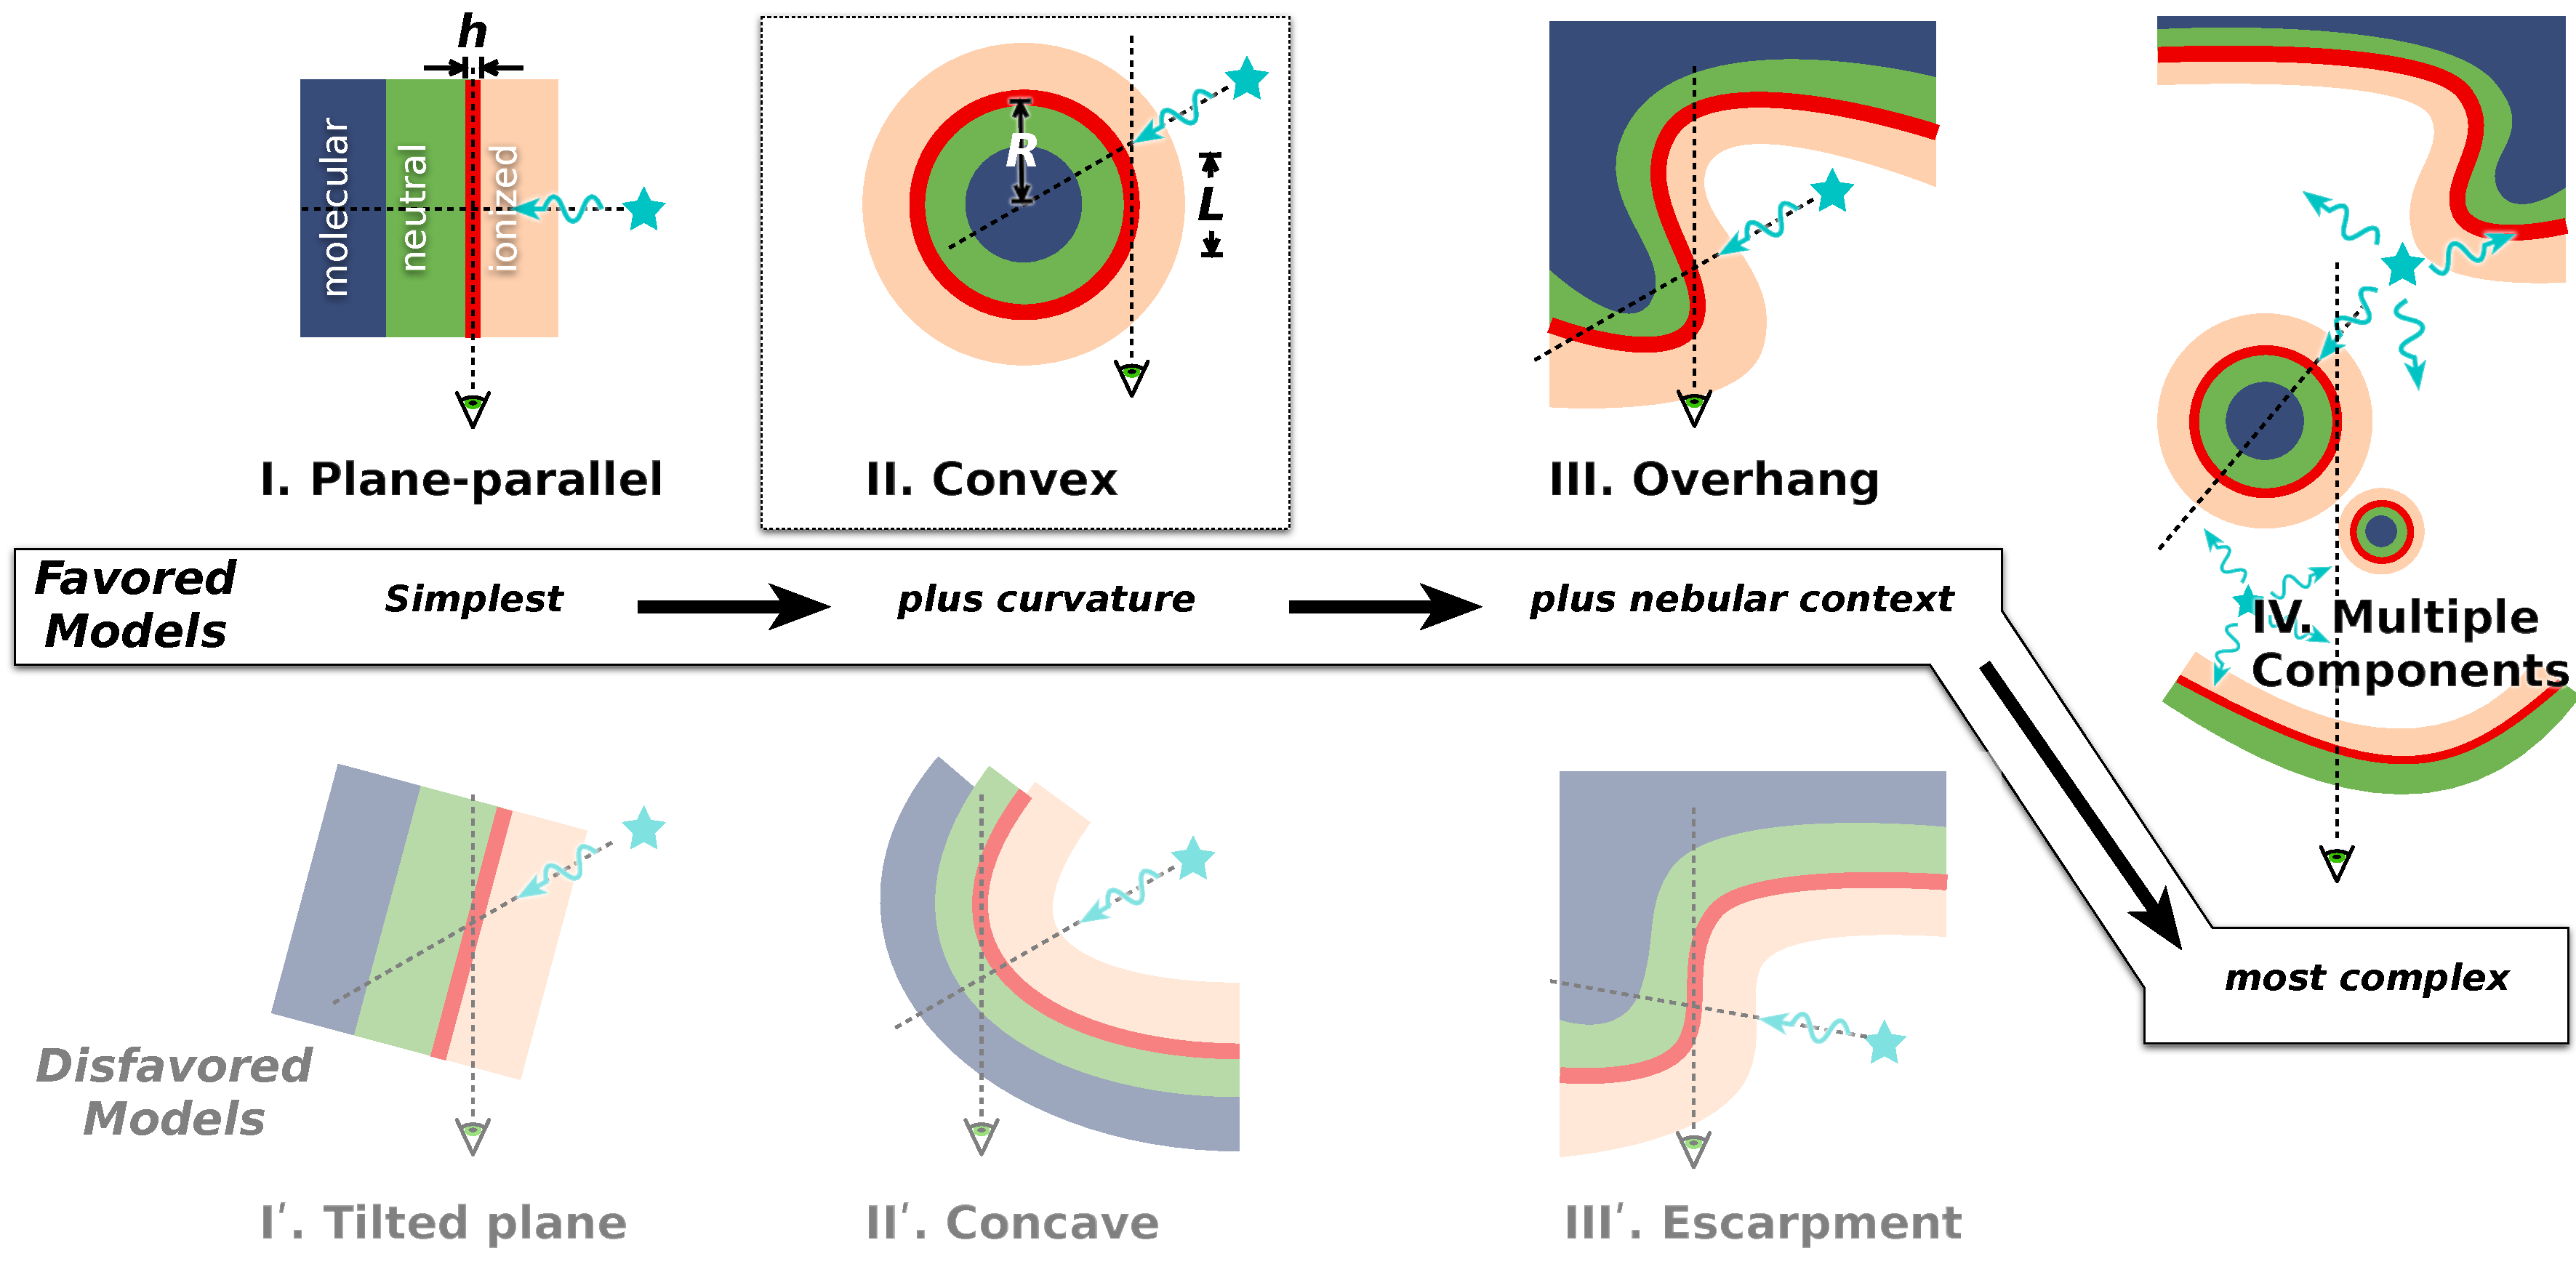
\includegraphics[width=\linewidth]{figs/bar-geometry-options}
  \caption{Different classes of geometrical models that have been
    proposed for the Orion Bar.  The sequence of models I, II, III, IV
    are of increasing complexity, but also increasing scope and
    explanatory power.  Models I\('\), II\('\), III\('\), on the other
    hand, are disfavored due to either underperformance or
    falsification (see text for further details).  For all models,
    dark blue shading represents molecular gas, green shading
    represents neutral gas, and light orange shading represents
    ionized gas.  An example emission layer of thickness \(h\) and
    radius of curvature \(R\) is indicated by thick red lines.  The
    line-of-sight depth of the emission layer is denoted by \(L\).
    The direction of illumination and the line of sight are indicated
    by thin dotted lines.  }
  \label{fig:bar-geometry}
\end{figure*}

\begin{figure*}
  \includegraphics[width=\linewidth]{figs/orion-bar-oi-hst-zoom}
  \caption{Fine-scale structure of the ionization front at the Orion Bar.
    Grayscale image shows a \(90'' \times 90''\) section of a mosaic of
    \textit{HST} WFPC2 observations \citep{Bally:2000a} in the F631N filter,
    which mainly passes the [\ion{O}{1}] \SI{6300}{\angstrom} line.
    The image has been high-pass filtered to remove large-scale brightness gradients
    (\(> \SI{16}{arcsec}\)).
    The principal ionization front of the Bright Bar runs diagonally from top-left to bottom-right.
    It can be seen that the front is very irregular on scales of \num{1} to \SI{10}{mpc},
    and even becomes disrupted completely in some segments.
    Only in a few places is the front straight and regular enough for its true sharpness to be seen,
    such as the small area shown in a zoomed box, where the width of the [\ion{O}{1}] ridge
    can be seen to be less than \SI{1}{mpc}.
    Apart from the Bright Bar ionization front,
    other fine-scale features visible in the image are associated with
    Herbig--Haro jets and proplyds.
  }
  \label{fig:bar-oi-hst}
\end{figure*}

\begin{figure*}
  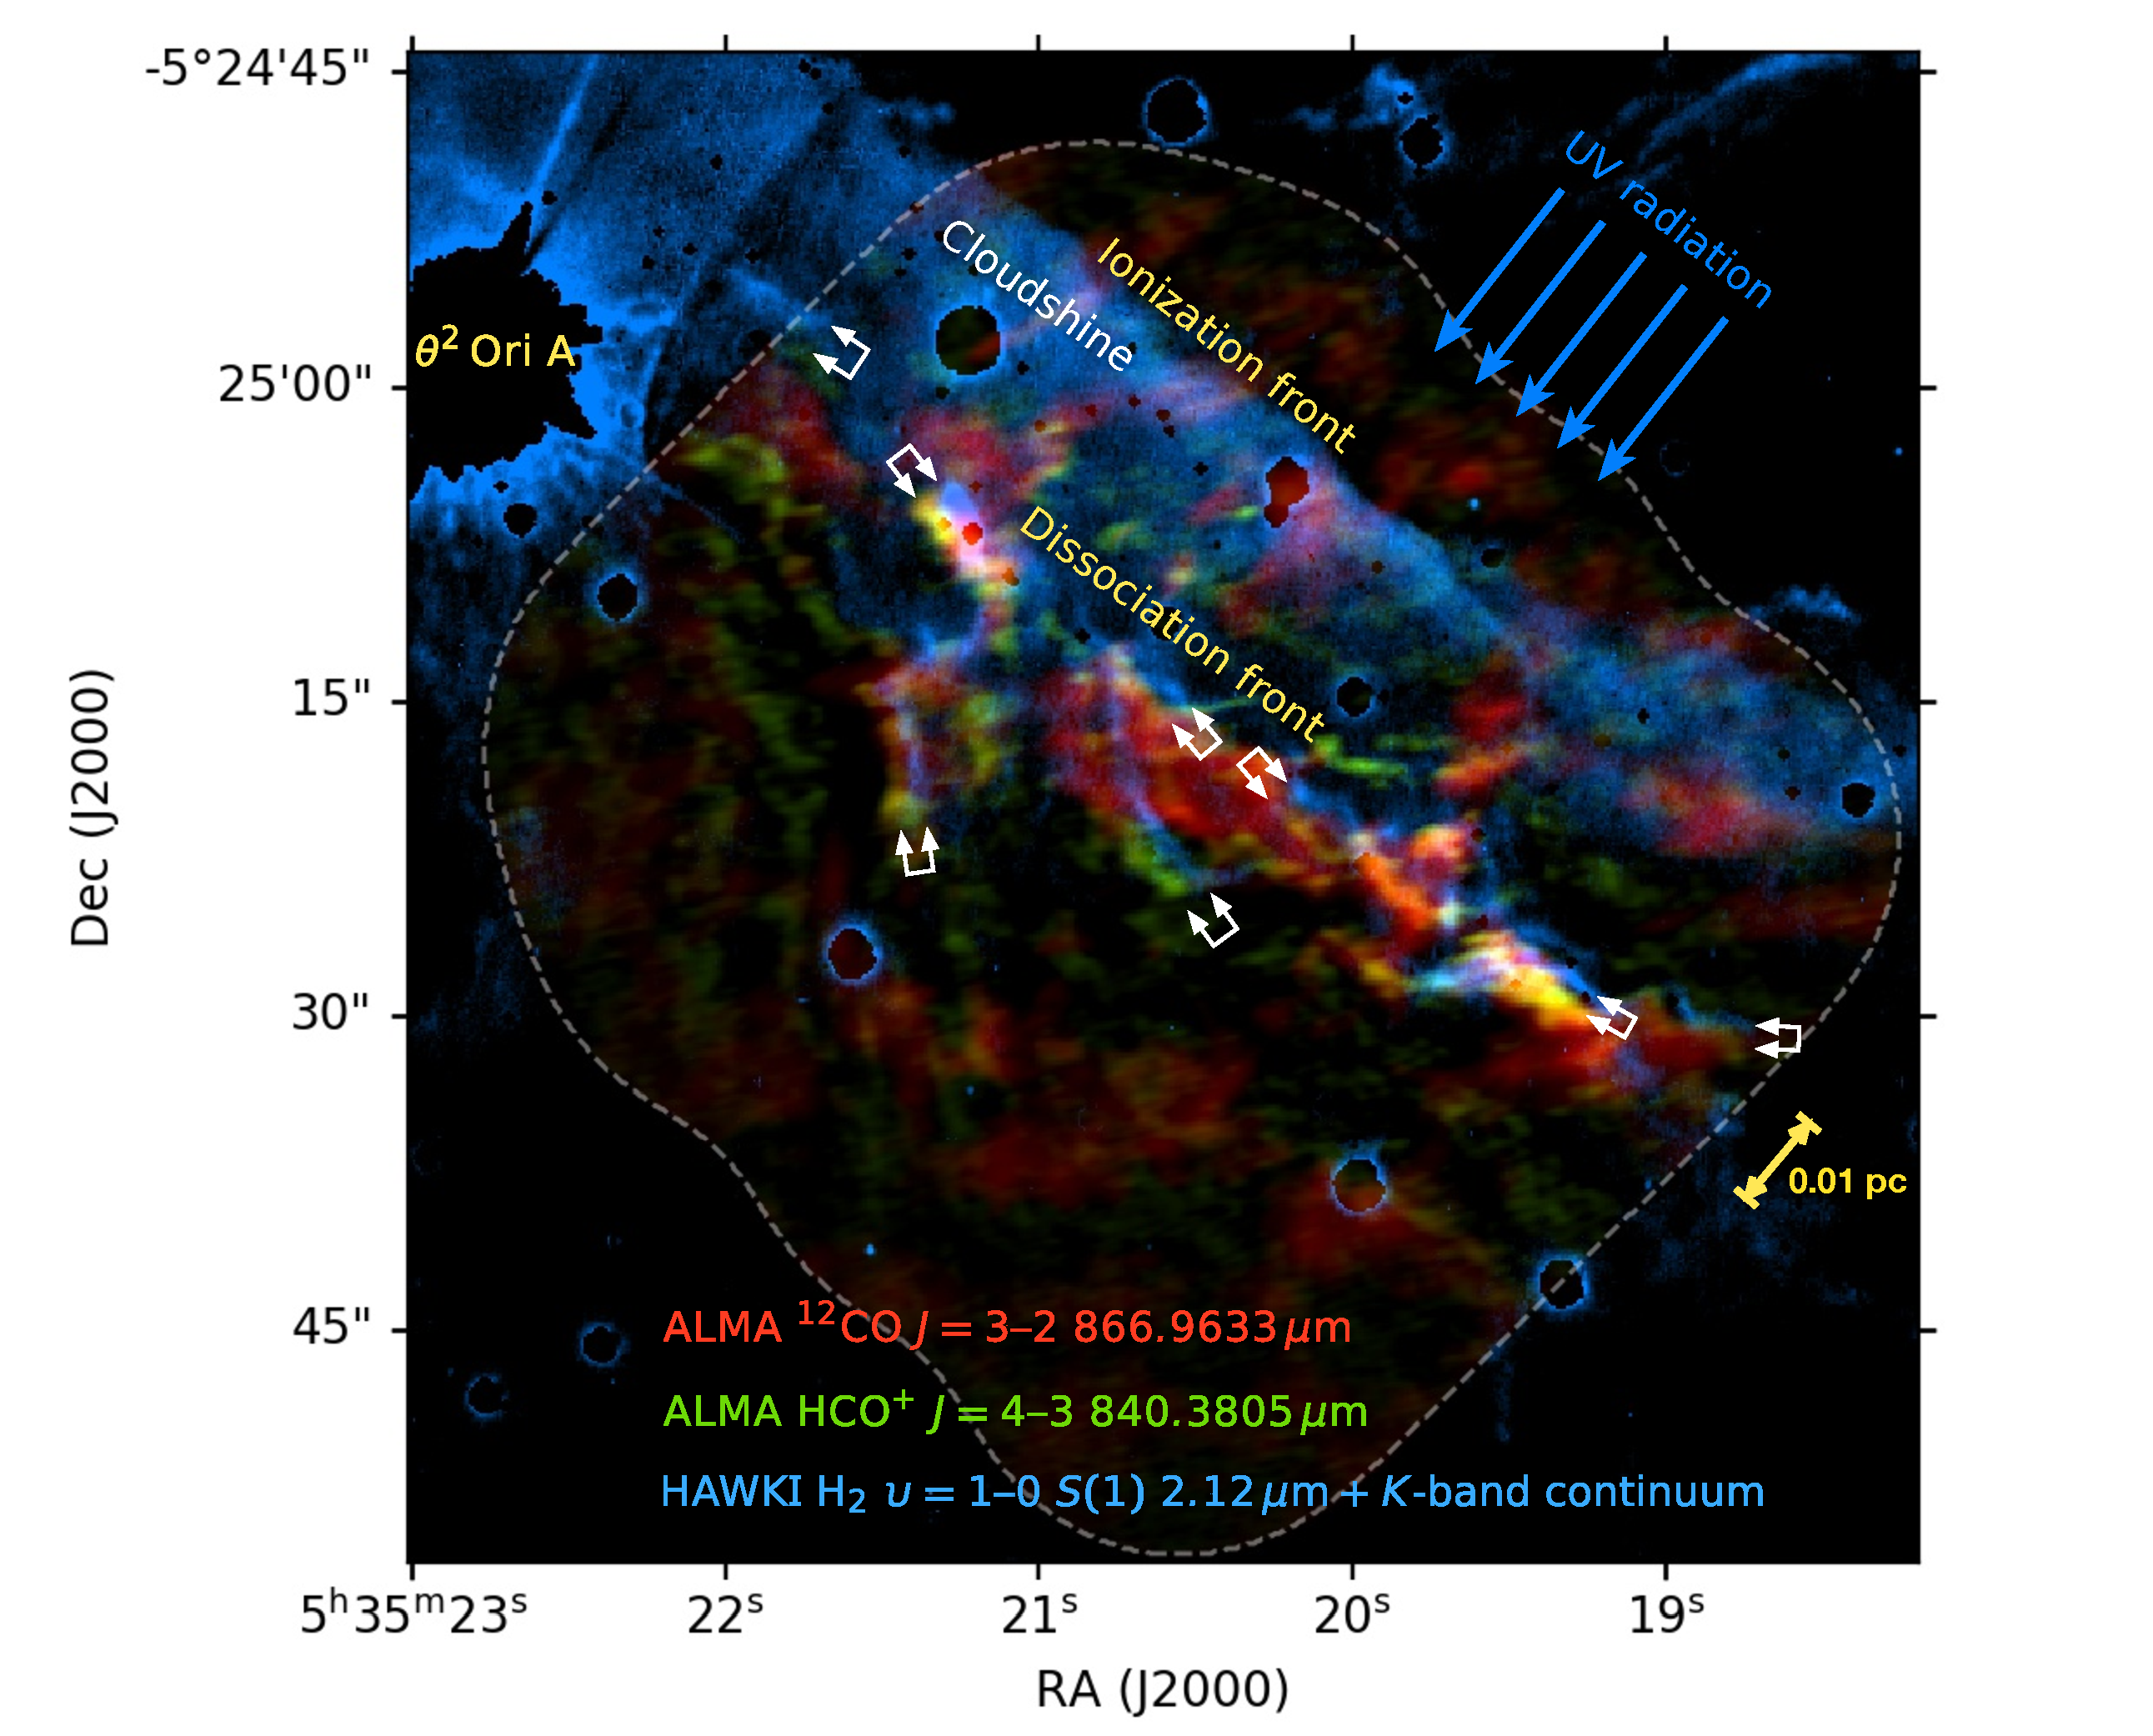
\includegraphics[width=\linewidth]{figs/alma-co-hcop-h2-dissoc-front}
  \caption{Fine-scale structure of the dissociation front in the Orion
    Bar.  Double white arrows mark out some instances of
    stratification between emission of \chem{H_2} (blue) and heavier
    molecules (green/yellow/red). In every instance \chem{H_2} is
    displaced towards the irradiated side of the filament by \(1''\)
    to \(2''\) (\(\approx \SI{0.003}{pc}\)).  Background image shows ALMA
    mosaics \citep{Goicoechea:2016a} of the sub-mm \chem{CO}
    \(J = 3 \to 2\) \SI{866.96}{\micron} \chem{HCO^+}
    \SI{840.38}{\micron} emission lines in the red and green color
    channels, respectively, with the boundary of the ALMA field shown
    by the gray dashed line. The blue color channel of the background
    image shows near-infrared vibrationally excited \chem{H_2}
    \(v = 1 \to 0\ S(1)\) \SI{2.12}{\micron} emission, extracted from
    narrow-band imaging with ESO's High Acuity Wide-field K-band
    Imager \citetext{HAWK-I, \citealp{Kissler-Patig:2008a}}. The
    \chem{H_2} image has been corrected for contamination by ionized
    emission (mainly hydrogen Br\(\gamma\) recombination line), but has not
    been continuum-subtracted.  As a result, scattered starlight
    \citetext{cloudshine, \citealp{Foster:2006a}} is seen as a band
    of diffuse emission that falls off smoothly behind the ionization
    front. }
  \label{fig:alma-dissoc-front}
\end{figure*}

\begin{figure}
  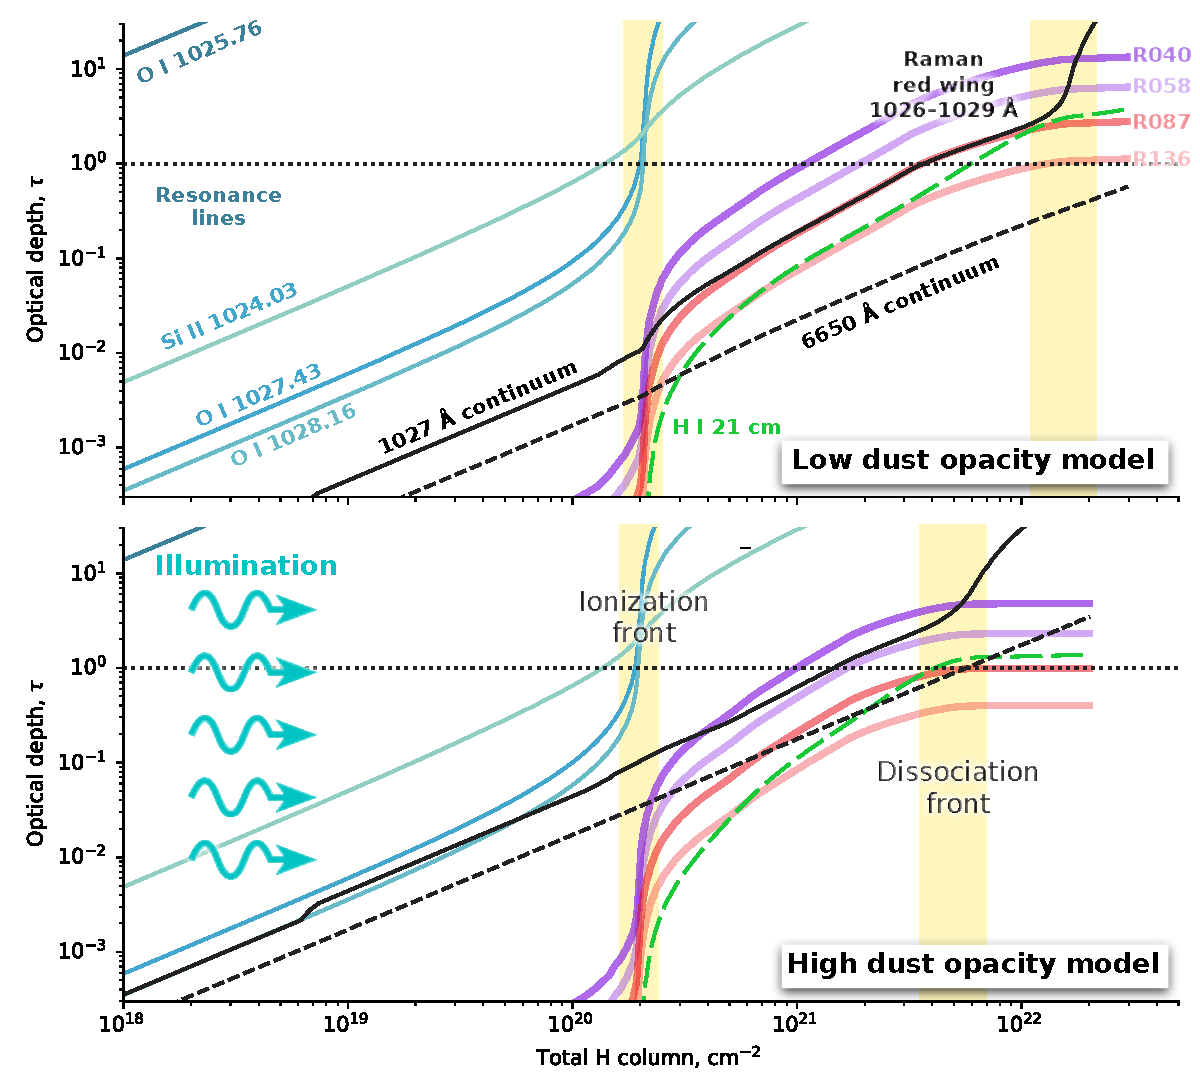
\includegraphics[width=\linewidth]{figs/cloudy-bar-optical-depths}
  \caption{Optical depth of select processes as a function of total
    hydrogen nucleon column density, calculated from static Cloudy
    simulations of the Orion Bar.  All optical depths and columns are
    measured with respect to the illuminating Trapezium stars, which
    are situated to the left in this figure.  Separate panels show two
    models that differ only in the assumed dust absorption opacity:
    (a)~low opacity, \(\sigma\FUV \approx \SI{5e-23}{cm^2.H^{-1}}\), and (b)~high
    opacity, \(\sigma\FUV \approx \SI{5e-22}{cm^2.H^{-1}}\). Optical depths of
    \chem{O^0} and \chem{Si^+} absorption lines in the \lyb{} wings
    are shown in blue. Continuum optical depths near \lyb{} (solid
    line) and \ha{} (dashed line) are shown in black.  The \chem{H^0}
    \SI{21}{cm} line optical depth is shown in green (long dashed
    line).  Optical depths to Rayleigh/Raman scattering for 4 observed
    bands in the red wing of \lyb{} (see Table~\ref{tab:wav-bands})
    are shown in red.}
  \label{fig:cloudy-bar-optical-depths}
\end{figure}
\begin{figure}
  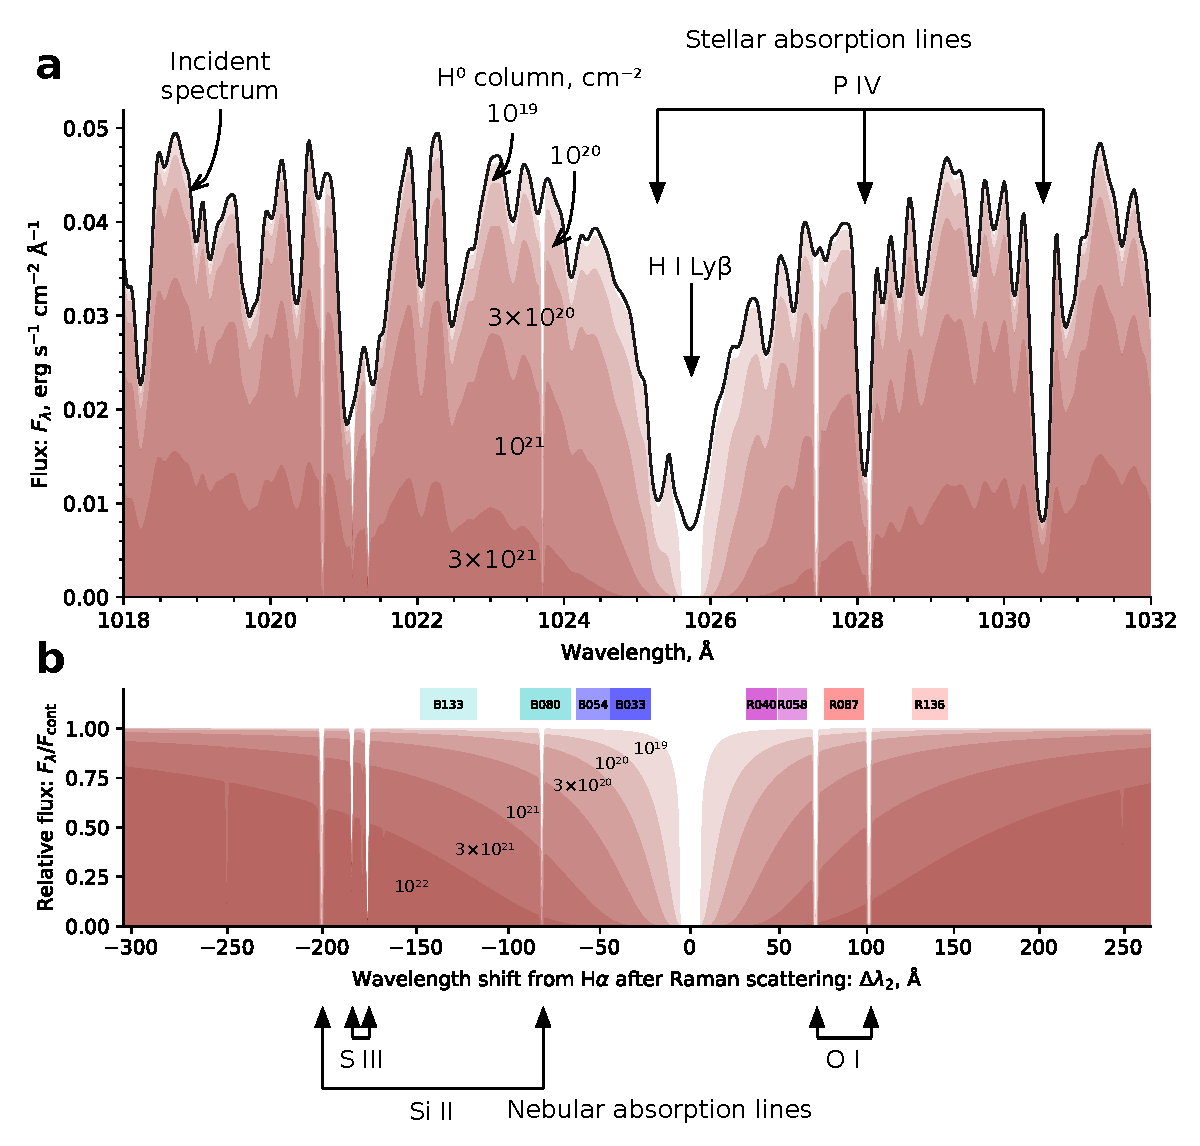
\includegraphics[width=\linewidth]{figs/stellar-spectrum-fuv}
  \caption{(a) Predicted spectrum of Trapezium stars in vicinity of
    \lyb{} from POWR OB atmosphere models (black line), together with
    attenuation by Cloudy model of the Orion Bar (red filled shapes),
    extracted at a series of values of the neutral hydrogen column
    density, as marked. (b) Relative attenuation of the incident
    spectrum by line opacity only (that is, neglecting dust continuum
    opacity) in the Cloudy models, which shows the development of the
    \lyb{} damping wings as the column density increases.  In this
    panel, the \(x\) axis is labelled with \(\Delta\lambda_2\) in the optical
    domain, allowing direct comparison with the observations presented
    in Figure~\ref{fig:raman-compensated} (observed Raman bands are
    indicated by colored boxes). Note that the scale is linear in
    \(\lambda_1\), which is slightly non-linear in
    \(\Delta\lambda_2\).  Wavelengths of some of the more prominent stellar
    photospheric lines and nebular absorption lines are marked. }
  \label{fig:stellar-spectrum-fuv}
\end{figure}



\subsubsection{Cloudy model predictions for the optical depths}
\label{sec:cloudy-model-pred}

In order to investigate the role of dust extinction in greater detail
in more detail the 

\textbf{Maybe ditch this section}
 


\bibliography{BibdeskLibrary}


\end{document}
%%% Local Variables:
%%% mode: latex
%%% TeX-master: t
%%% End:
